%% LyX 2.0.5.1 created this file.  For more info, see http://www.lyx.org/.
%% Do not edit unless you really know what you are doing.
\documentclass[usenatbib]{article}
\usepackage[latin9]{inputenc}
\usepackage[a4paper]{geometry}
\geometry{verbose}
\usepackage{color}
\usepackage{verbatim}
\usepackage{float}
\usepackage{graphicx}

\makeatletter

%%%%%%%%%%%%%%%%%%%%%%%%%%%%%% LyX specific LaTeX commands.
%% Because html converters don't know tabularnewline
\providecommand{\tabularnewline}{\\}
%% A simple dot to overcome graphicx limitations
\newcommand{\lyxdot}{.}


%%%%%%%%%%%%%%%%%%%%%%%%%%%%%% Textclass specific LaTeX commands.
\usepackage{jcappub}

%%%%%%%%%%%%%%%%%%%%%%%%%%%%%% User specified LaTeX commands.






%%%%%%%%%%%%%%%%%%%%%%%%%%%%%% LyX specific LaTeX commands.
%% A simple dot to overcome graphicx limitations
%Make my life significantly easier
\global\long\def\bd{{\bm{\delta}}}

\makeatother

\begin{document}

\title{The Maximum Circular Velocity Dependence of Halo Clustering}

\maketitle

\section{Introduction}

The halo model has been remarkably successful in describing observations
of galaxy clustering at many scales and many redshifts (give some
examples here). fundamental assumption clustering only depends on
the halo mass; not true because of assembly bias on large scales but
also ideas of e.g.. backsplashed halos. recent trend has been to populate
galaxies according to their maximum circular velocity. Describe why
this might be motivated \textemdash{} depends only on the central
part of the potential, set early in the growth of the halo (point
to Frank\textquoteright{}s recent paper here as an example). Also
may be more robust to disruption in mergers.

goal here is to discuss the dependence of galaxy clustering on the
central velocity dispersion both on small and large scales. We show
that some of the features in a detailed halo model come from the effects
of back-splash halos.


\section{The Simulation}

We use cosmological N-body simulations called the Bolshoi simulation
and the MultiDark simulation, described in XXX and XXX respectively,
to investigate the maximum circular velocity dependence of halo clustering.
The Bolshoi simulation uses $2048^{3}$ particles with a volume of
$(250$$h^{-1}{\rm Mpc})^{3}$, while the MultiDark simulation uses
the same number of particles as the Bolshoi simulation but with a
volume of ($1h^{-1}{\rm Gpc})^{3}$. Both simulations assumes a flat
$\Lambda{\rm CDM}$ model with density parameters $\Omega_{m}=0.27$,
$\Omega_{\Lambda}=0.73$, $\Omega_{b}=0.0469$, and $\sigma_{8}=0.82$,
$n=0.95$, $h=0.70$. The details of the simulations are described
in XXX. We use both simulations to get large dynamic mass range.

For halo identification, we use the ROCKSTAR halo finder (XXX) where
the halo masses and maximum circular velocities are computed from
bound particles. For the sake of internal structure of halos to be
resolved well enough, we make very conservative cut in mass and maximum
circular velocity. We use halos whose mass is greater than $10^{12}h^{-1}{\rm M_{\odot}}$
(corresponding to $>100$ particles per halo) and whose maximum circular
velocity is greater than $200{\rm km/s}$ for the MultiDark simulation
and halos whose mass is greater than $10^{11}h^{-1}{\rm M_{\odot}}$
(corresponding to $>740$ particles per halo) and whose maximum circular
velocity is greater than $95{\rm km/s}$ for the Bolshoi simulation.
Those values correspond to the peak in the number of halos by binning
them as a function of mass and maximum circular velocity. The ROCKSTAR
halo finder also provides the merger trees for halos classified into
three different categories of halos: host halo, subhalos, and ejected
halos. Host halos are the halos which never been within the virial
radius of more massive halos. Subhalos are the halos which are within
the virial radius of more massive halos at $z=0$. Ejected halos,
sometimes called ``backsplash'' halos, are the distinct halos at
$z=0$ whose main progenitor passed through the virial radius of a
more massive halos at least once in the past.


\section{The Maximum Circular Velocity Dependence of Halo Clustering}

In this section, we investigate the maximum circular velocity dependence
of halo clustering on both large and small scales. We first start
with an analytic expression of the maximum circular velocity computed
from the halo mass and its concentration. Then, we explain how we
select halos to remove the halo mass dependence from the samples using
the analytic expression of the maximum circular velocity.


\subsection{The Maximum Circular Velocity}

Here, we assume that dark matter halos are defined as a spherical
halo with a virial radius. Those halos have average density equal
to $\Delta_{{\rm h}}\rho_{{\rm crit}}$ where $\Delta_{{\rm h}}=360$
for the MultiDark and Bolshoi simulations. We also assume that those
spherical halos have an NFW density profile (XXX). Then, the maximum
circular velocity $\overline{V}_{{\rm max}}$ as a function of the
halo mass $M_{{\rm vir}}$ and its concentration $c$ is given by:

\begin{equation}
\overline{V}_{{\rm max}}=0.465M_{{\rm vir}}^{1/3}\sqrt{G(\frac{4}{3}\pi\Delta_{{\rm h}}\rho_{{\rm crit}}\Omega_{m})^{1/3}\frac{c}{{\rm ln(1+c)-c/(1+c)}}}.\label{eq:vmax-mvir}
\end{equation}
The median concentration-mass relation at $z=0$ obtained from the
Bolshoi simulation in Ref. XXX(Klypin et al. 2011) is: 
\begin{equation}
{\rm log}_{10}c=-0.097{\rm log_{10}M_{vir}}+2.148.\label{eq:concen}
\end{equation}
\textcolor{black}{By using the above median concentration to Eq. \ref{eq:vmax-mvir},
we obtain a one to one mapping between the virial halo mass and its
maximum circular velocity, denoted as $\overline{V}_{{\rm max}}$
hereafter.} Given this mapping, we can translate clustering measurements
as a function of halo mass into predicted clustering measurements
as a function of maximum circular velocity. Our goal below is to determine
whether this conversion describes the measured clustering or if there
is a residual dependence on the maximum circular velocity.


\subsection{Samples}

\begin{figure}
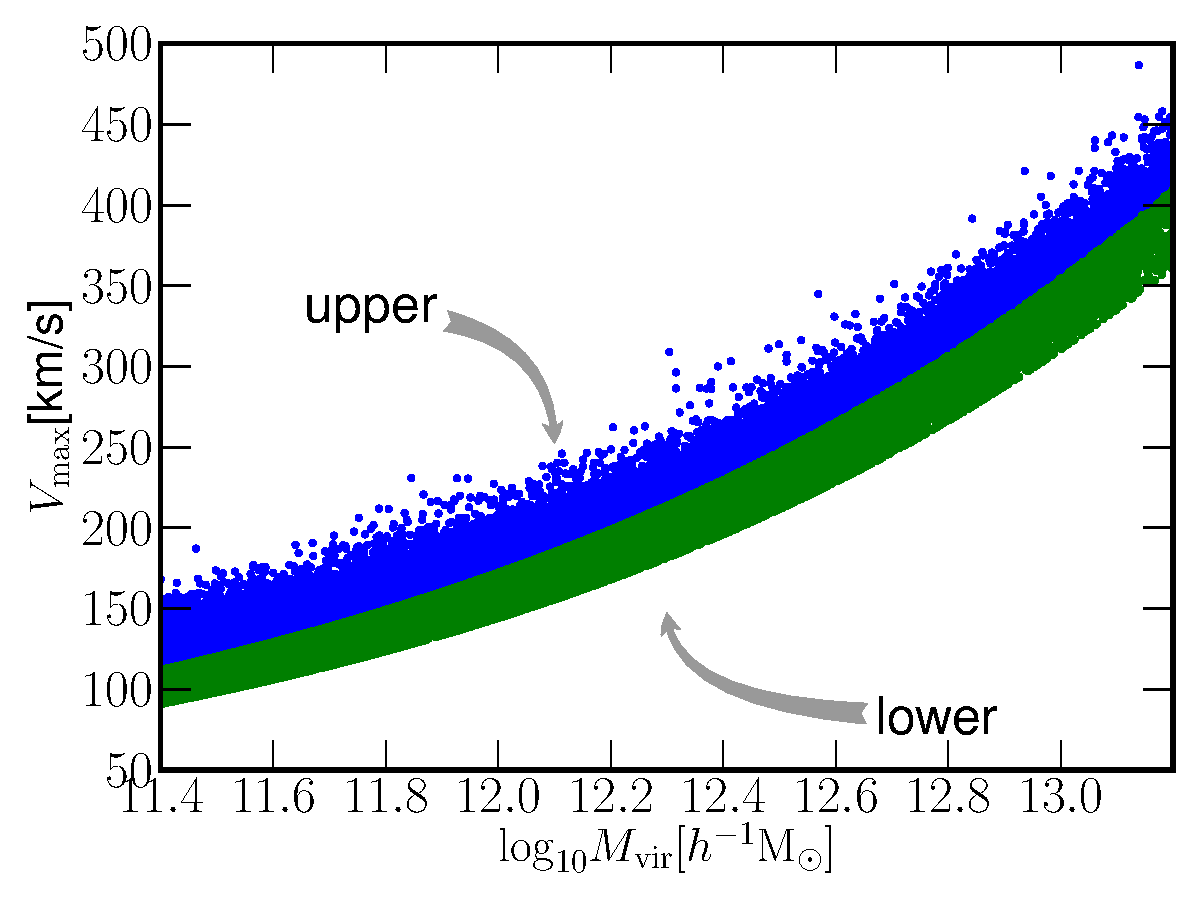
\includegraphics[width=0.5\columnwidth]{/Users/old_ts485/Desktop/biasVmax/plots/logVmax_logMvir_Dh360}\caption{\label{fig:vmax-mvir}Distribution of halo mass and maximum circular
velocity at $z=0.0$ for halos\textcolor{black}{{} from the Bolshoi
simulation.} The blue dots represent halos whose observed maximum
circular velocity, $V_{{\rm max,obs}}$, is greater than $\overline{V}_{{\rm max}}$,
while the green dots are the ones with smaller $V_{{\rm max,obs}}$
than $\overline{V}_{{\rm max}}$. The boundary between blue and green
dots correspond to $\overline{V}_{{\rm max}}$ computed from Eq. \ref{eq:vmax-mvir}.}
\end{figure}


In order to explore a dependence on the maximum circular velocity,
we first split the sample into a sequence of virial mass bins, chosen
such that there are the same numbers of halos in each bin. This process
is reminiscent of an abundance-matching procedure (cite XXX). We then
further split each bin into two subsamples with their observed $V_{{\rm max,obs}}$
greater than (denoted by ``upper'') or less than (denoted as ``lower'')
$\overline{V}_{{\rm max}}$. Fig. \ref{fig:vmax-mvir} shows the distribution
of halo mass and maximum circular velocity classified into ``upper''
(blue dots) and ``lower'' (green dots) samples as an example. As
you can see, the number of halos in each sample is almost half for
any halo mass bins. This selection ensures that both the upper and
lower subsamples have the same mean halo mass. Therefore, in the absence
of an additional $M_{{\rm vir}}$ dependence on clustering, these
samples should have the same clustering properties. Note that this
would not be true if we had simply split the sample along $V_{{\rm max}}$,
since the two resulting subsamples would have different mean halo
masses. 


\subsection{Halo Bias}

We use cross correlation functions to reduce the shot noise effect
on the error. In order to measure halo biases, we compute halo-matter
cross correlation functions for each subsample and measure a linear
bias 
\begin{equation}
b_{{\rm lin}}=\sum_{i}(\xi_{hm}(r_{i})/\xi_{mm}(r_{i}))/N_{{\rm bin}},
\end{equation}
where $\xi_{hm}$ and $\xi_{mm}$ are halo-matter and matter-matter
correlation functions and we take the average of the ratio on $r$
from $10h^{-1}{\rm Mpc}$ to $20h^{-1}{\rm Mpc}$, which contains
20 bins as a total. Here, instead of using full DM particles, we subsample
$1000000$ particles to compute matter auto correlation functions. 

In Fig. \ref{fig:linear-bias}, we show how linear biases depend on
the maximum circular velocity as a function of halo mass. We compute
linear biases for each mass bin classifying into ``upper'' and ``lower''
maximum circular velocity halos. The halos which have different maximum
circular velocity have different linear bias values. On large mass
end, halos with $V_{{\rm max}}<\overline{V}_{{\rm max}}$ have a larger
linear bias, which is consistent to the result discussed in Ref. XXX(Dalal
et al. 2008). On the other hand, as halo masses decrease, halos with
$V_{{\rm max}}>\overline{V}_{{\rm max}}$ start having larger linear
biases than those with $V_{{\rm max}}<\overline{V}_{{\rm max}}$,
and the difference between those two samples increases up to 40\%.
We think that the drop of the ratio on the low mass end is due to
mass resolution of the simulation not resolving all the halos\textcolor{black}{{}
for the low mass}.

\begin{comment}
things that I want to write (possibly with the histogram): Halos which
have larger maximum circular velocity than the one predicted from
its halo mass have high concentration. Those halos which have high
concentration are the halos which should have grown to larger halo
mass but somehow the mass growth was suppressed or its mass was stripped
from other larger halos...want to explain things more clearly...any
good papers which explain about this physical picture?
\end{comment}


\begin{figure}
\includegraphics[width=0.5\columnwidth]{/Users/old_ts485/Desktop/biasVmax/plots/linearBias_wang}

\caption{\label{fig:linear-bias}Upper panel: Linear bias at $z=0.0$ as a
function of halo mass from the Bolshoi simulation and the MultiDark
simulation. The blue circles corresponds to a linear bias for halos
whose maximum circular velocities are greater than $\overline{V}_{{\rm max}}$
(called ``upper'' samples in the text), while the green circles
correspond to halos whose maximum circular velocities are smaller
than $\overline{V}_{{\rm max}}$ (called ``lower'' samples). Lower
panel: Ratio of linear biases between ``upper'' (i.e., $V_{{\rm max}}>\overline{V}_{{\rm max}}$)
and ``lower'' (i.e., $V_{{\rm max}}<\overline{V}_{{\rm max}}$)
samples from the Bolshoi simulation and the MultiDark simulation.
As halo masses decrease, the difference on linear bias between ``upper''
and ``lower'' samples becomes larger up to 40\%. .}
\end{figure}


In Fig. \ref{fig:small-scale}, we investigate the maximum circular
velocity dependence of halo bias on small scales. On small scales,
a halo bias is scale-dependent. The question here is whether halos
with different maximum circular velocity have different scale-dependence
on their biases. In order to find that, we take the ratio of halo-matter
cross correlation functions between ``upper'' and ``lower'' subsamples
and normalize it by their linear biases, shown in Fig. \ref{fig:small-scale}.
By normalizing by their linear biases, the ratios go to one on large
scales. Fig. \ref{fig:small-scale} clearly shows different scale-dependence
between ``upper'' and ``lower'' subsamples\textcolor{black}{,
and the difference becomes larger a}s halo masses decrease. We particularly
see that there is a characteristic bump around 1 to 2 $h^{-1}{\rm Mpc}$.
This implies that many halos in the ``upper'' samples, especially
low mass halos, cluster very closely to each other. 

Up to now, we use both host halos and ejected halos to compute halo
biases. Both types of halos are identified as distinct halos at $z=0$.
Ejected halos are, however, halos which were identified as a part
of a more massive halos at one or more occasions in the past. Those
ejected halos tend to exist around a more massive halos (any reference?),
and only some of them may be gravitationally bound to other more massive
halos. We question how much of the effect in the scale-dependent biases
is caused by those ejected halos.

To test this, we compute halo-matter cross correlation functions without
the ejected halos. Fig. \ref{fig:eject} shows the same figures as
Fig. \ref{fig:small-scale} without ejected halos from the Bolshoi
simulation. Due to mass resolution, we could not find many ejected
halos in the MultiDark simulation. \textcolor{black}{After removing
ejected halos, the ratios of linear biases between ``upper'' and
``lower'' samples are suppressed by \textasciitilde{}10\%. }\textcolor{red}{There
are, however, still more than 25\% differences in those samples. }\textcolor{black}{Once
removing the ejected halos, the deviation of the halo bias on small
scales is greatly reduced. }\textcolor{red}{On the other hand, the
different scale dependence of halo bias appeared on small scales significantly
goes down to less than 10\%, which implies that difference in small
scale halo biases are mostly due to the ejected halos.}

We conclude that halos which have different $V_{{\rm max}}$ cluster
differently even when those halos have the same virial mass. Especially,
the scale-dependence of halo biases on small scales shows a siginificant
difference, which mainly caused by the ejected halos.

\begin{comment}
Halos which have high $V_{{\rm max}}$ are the ones which could have
grown to a larger halo mass, but did not due to suppression of mass
growth caused by tidal fields in high density regions (any references
for this picture, and also how can I phrase this better?), and therefore
they have larger halo biases than the ones which low $V_{{\rm max}}$.
\end{comment}


\begin{figure}[H]
\includegraphics[width=0.8\columnwidth]{/Users/old_ts485/Desktop/biasVmax/plots/Both_smallScale_wang_log}

\caption{\label{fig:small-scale}Ratio of halo-matter cross correlation functions
between ``upper'' and ``lower'' subsamples normalized by their
linear biases. The plots are from the Bolshoi simulation and the MultiDark
simulation at z = 0.0. Each line corresponds to different halo mass
bins labeled in the plots. Those plots show that ``upper'' and ``lower''
subsamples have different scale-dependence on small scales and the
relative scale-dependence between those subsamples increases smoothly
with decreasing halo mass. }


\end{figure}


\begin{figure}[H]
\includegraphics[width=0.5\columnwidth]{/Users/old_ts485/Desktop/biasVmax/plots/Bolshoi_smallScale_wang_log_eje}

\caption{\label{fig:eject}The same figures as Fig. \ref{fig:small-scale}
without ejected halos from the Bolshoi simulation. As can be seen
by comparing these results to those in Fig. \ref{fig:small-scale},
the Vmax-dependence of halo bias on small scales is dramatically reduced
by excluding ejected subhalos. This implies an intimate connection
between assembly bias and subhalo back-splashing.}


\end{figure}


--use jackknife sampling to put error bars


\section{Applications}

In this section, we demonstrate possible observational relevances
of the results in the previous section to complement the halo theory
results. We start with the abundance matching (citation?) technique
based on halo mass and the maximum circular velocity, and then compute
$\Delta\Sigma({\rm R})$ using those two different abundance matching.


\subsection{Mvir-based v.s. Vmax-based}

In abundance matching, we assume that a big galaxy lives in a big
halo in a hierarchical manner to link galaxies to halos. The question
is what ``big'' halos really mean. To rank order halos, we want
to identify what kind of physical properties of halos characterize
``size'' of halos. As a first step, we explore how the abundance
matching based on halo mass and maximum circular velocity make difference
on halo clustering.

First, we check the correspondence between $\overline{n}(M_{{\rm vir}})$
and $\overline{n}(V_{{\rm max}})$ as shown in Fig. \ref{fig:nbar}.
The red line shows the boundary where $\overline{n}(M_{{\rm vir}}<)=\overline{n}(V_{{\rm max}}<)$
(how can I phrase this differently?). This boundary overlaps with
$\overline{V}_{{\rm max}}$ from Eq. \ref{eq:vmax-mvir}, which implies
that XXX. 

Similar to the previous section, we compute halo-matter cross correlation
functions for the abundance matched samples by splitting halos into
a sequence of halo mass bins and the maximum circular velocity bins
chosen such that each bin has the same number of halos. We observe
that the linear biases for the samples $\overline{n}(V_{{\rm max}})$
are larger than the ones for the samples $\overline{n}(M_{{\rm vir}})$
by 5\% with ejected halos, while the difference in linear biases is
suppressed to 2\% by excluding ejected halos. This result agrees with
the result in Sec. 3.2. The magnitude of the difference is, however,
smaller than the cases of splitting the samples based on $\overline{V}_{{\rm max}}$. 

We also compare the cross correlation functions on small scales. Figure
\ref{fig:abundance_small} is the same as Figure \ref{fig:small-scale}
with the ejected halos (left panel) and without the ejected halos
(right panel). We see the same trend as the previous section in the
different scale dependence between $\overline{n}(M_{{\rm vir}})$
and $\overline{n}(V_{{\rm max}})$, which is caused mainly by the
ejected halos.

--how to describe the result for small scale biases?

--interpretation/implication

--what's the possible problem if any

--what's interesting

--check the number of ejected halos in Vmax and Mvir:

\begin{figure}[H]
\includegraphics[width=0.5\columnwidth]{/Users/old_ts485/Desktop/biasVmax/plots/logMhalo_Vcir_nbar_Bolshoi}

\caption{\label{fig:nbar}Distribution of halo mass and the maximum circular
velocity as a contour plot, overplotted $\overline{V}_{{\rm max}}$
(as a green dashed line) and the correspondence between $M_{{\rm vir}}$
and $V_{{\rm max}}$ in abundance matching (as a red dashed line labeled
as $\overline{n}$). The plot shows that $\overline{V}_{{\rm max}}$
and the correspondence in abundance matching overlaps on most of halo
mass scales.}


\end{figure}


\begin{figure}[H]
\includegraphics[width=0.5\columnwidth]{/Users/old_ts485/Desktop/biasVmax/plots/Bolshoi_andrew_smallScale}\includegraphics[width=0.5\columnwidth]{/Users/old_ts485/Desktop/biasVmax/plots/Bolshoi_andrew_smallScale_nonEj}

\caption{\label{fig:abundance_small}Ratio of halo-matter cross correlation
functions between$M_{{\rm vir}}$-based and $V_{{\rm max}}$-based
abundance matching samples with ejected halos (left) and without ejected
halos (right). The ratios are normalized by their linear biases. Each
line corresponds to different halo mass bins labeled in the plots
(which can be translated into corresponding $\overline{V}_{{\rm max}}$
through Eq. \ref{eq:vmax-mvir}). When samples contain ejected halos,
there is a strong scale-dependent difference between those two different
abundance matching samples around $1h^{-1}{\rm Mpc}$. By excluding
ejected halos, the difference is more or less removed.}
\end{figure}


\begin{figure}
\includegraphics[width=0.5\columnwidth]{/Users/old_ts485/Desktop/biasVmax/plots/num_eject}

\caption{The number of ejected halos as a function of halo mass (need to change
either y-label or the plotted object). }


\end{figure}



\subsection{$\Delta\Sigma(r)$}

(Both are from Andrew's comments)

--Select a bin of Milky Way mass host halos, and select their number-density-matched
Vmax-selected equivalent. Use Peter Behroozi's stellar-to-halo mass
relation to estimate the stellar mass of the central galaxy that would
be found in these halos, then plot the halo-matter cross-correlation
as a function of scale, over-plotting the two results.

--want to show: We show that the galaxy-galaxy lensing signal of low-mass
centrals is impacted at the xxx-yyy\% level, in a highly scale-dependent
fashion, by the theoretical choice to empirically connect stellar
mass to either host halo Vmax or Mvir.


\subsection{HOD(?)}


\section{Discussion}

(Option)

\begin{figure}
\includegraphics[height=0.5\columnwidth]{/Users/old_ts485/Desktop/biasVmax/plots/linearBias_andrew_Bolshoi}\includegraphics[height=0.5\columnwidth]{/Users/old_ts485/Desktop/biasVmax/plots/linearBias_andrew_Bolshoi_nonEj}\caption{\label{fig:abundance_linear}Upper panel: We compare linear biases
for halos selected by abundance matching for halo mass (blue dots)
and the maximum circular velocity (green dots) as a function of halo
mass. As shown in Fig. \ref{fig:nbar}, we can find a corresponding
$V_{{\rm max}}$ for those samples through Eq. \ref{eq:vmax-mvir}.
The left panel is the result including ejected halos, while the right
panel is the one without ejected halos. The linear biases overall
decrease by excluding ejected halos for both $M_{{\rm vir}}$-based
and $V_{{\rm max}}$-based abundance matching samples. Lower panel:
Ratio of linear biases between $M_{{\rm vir}}$-based and $V_{{\rm max}}$-based
abundance matching samples with ejected halos (left) and without ejected
halos (right). The difference between those samples become smaller
by at most factor of 2.}
\end{figure}


\begin{figure}[H]
\includegraphics[width=0.5\columnwidth,bb = 0 0 200 100, draft, type=eps]{/Users/old_ts485/Downloads/dist2_nearestCluster_m11.7to11.8.pdf}

\caption{Histogram of distances to the nearest Clusters (defined as $M_{vir}>10^{14}{\rm M_{\odot}}$)
for non-ejected halos and ejected halos: Right now, I only have the
one for all the halos...may change to the plot of fractions: Is it
reasonable to play with the cluster masses? Also, make the similar
plots for nearest massive halos by separating ejected and non-ejected
halos (upper/lower)...}
\end{figure}


\begin{table}
\begin{tabular}{|c|c|c|c|}
\hline 
 & Mvir & Vmax & Vmax/Mvir\tabularnewline
\hline 
\hline 
0 & 1669 & 1730 & 1.037\tabularnewline
\hline 
1 & 1838 & 2041 & 1.110\tabularnewline
\hline 
2 & 2056 & 2352 & 1.144\tabularnewline
\hline 
3 & 2418 & 2623 & 1.085\tabularnewline
\hline 
4 & 2553 & 2732 & 1.070\tabularnewline
\hline 
5 & 2684 & 3098 & 1.154\tabularnewline
\hline 
6 & 2684 & 3161 & 1.178\tabularnewline
\hline 
7 & 2839 & 3435 & 1.210\tabularnewline
\hline 
8 & 2970 & 3458 & 1.164\tabularnewline
\hline 
9 & 3030 & 3673 & 1.212\tabularnewline
\hline 
\end{tabular}

\caption{number of ejected halos}
\end{table}

\end{document}
